% =====================================================================
%  Rapport final — Projet 1
%  Solveur de Nash m x n et duopoles (Cournot, Bertrand)
%  Groupe 1 — Théorie des Jeux et Systèmes Multi-Agents — ENSA Safi
%
%  Squelette à compléter au fil des semaines (viser 80 % en S6).
%  Compilation : pdflatex rapport.tex
%  Les zones « À COMPLÉTER » indiquent le contenu attendu.
% =====================================================================
\documentclass[11pt,a4paper]{article}

\usepackage[utf8]{inputenc}
\usepackage[T1]{fontenc}
\usepackage[french]{babel}
\usepackage{amsmath,amssymb}
\usepackage{geometry}
\usepackage{graphicx}
\usepackage{booktabs}
\usepackage{enumitem}
\usepackage{hyperref}

\geometry{margin=2.2cm}
\graphicspath{{../gantt/}{../}}
\usepackage{xcolor}
\hypersetup{colorlinks=true, linkcolor=blue, urlcolor=blue}

\newcommand{\todo}[1]{\textcolor{red}{[À COMPLÉTER : #1]}}

\title{\textbf{Rapport final — Projet 1}\\[4pt]
\large Solveur de Nash $m\times n$ et duopoles (Cournot, Bertrand)}
\author{Groupe 1 : ACHTOUK Fatine, ADIL Youness, BELHIMER Ikram, BOULHAIL Hiba\\
\small Cycle Ingénieur — Informatique Décisionnelle et IA (IDIA3)\\
\small Module : Théorie des Jeux et Systèmes Multi-Agents — ENSA Safi — Pr.\ A.\ JRAIFI}
\date{Année universitaire 2026--2027}

\begin{document}
\maketitle
\tableofcontents
\newpage

% ---------------------------------------------------------------------
\section{Introduction et problématique}
Le cours de Théorie des Jeux et Systèmes Multi-Agents introduit un solveur
\texttt{nash\_mixte\_2x2} limité aux jeux $2\times2$. Or la plupart des situations
économiques réelles (oligopoles, enchères, négociations) se modélisent par des jeux à
plus de deux stratégies. \textbf{Problématique :} comment généraliser le calcul des
équilibres de Nash à des jeux finis $m\times n$ quelconques, puis mettre ce calcul à
disposition d'un agent conversationnel (LLM local) qui traduit un énoncé en langage
naturel en un appel d'outil correct ?

Le projet répond en trois étapes : (i) un solveur exact par \emph{énumération des supports},
(ii) son application aux duopoles de \textbf{Cournot} et de \textbf{Bertrand}, (iii) son
exposition à l'agent LangChain du cours connecté au LLM local \texttt{llama3.1} via Ollama.
Le rapport décrit ensuite l'organisation, la théorie, la méthodologie, les résultats
expérimentaux et les écarts observés.

Le projet consiste à généraliser le solveur \texttt{nash\_mixte\_2x2} du cours en un solveur
d'équilibres de Nash pour jeux à deux joueurs de taille quelconque $m\times n$ par
\emph{énumération des supports}, puis à l'appliquer aux duopoles de \textbf{Cournot} et de
\textbf{Bertrand} et à l'exposer à l'agent LangChain du cours (LLM local Ollama).

% ---------------------------------------------------------------------
\section{Organisation et planification}
\subsection{Membres et rôles (semaines 1 à 4)}
\begin{center}
\begin{tabular}{lll}
\toprule
Membre & Rôle (S1--S4) & Rôle (S5--S7, après rotation) \\
\midrule
ACHTOUK Fatine & Chef de projet / Théorie & Testeur / Expérimentateur \\
ADIL Youness & Développeur agent & Chef de projet / Théorie \\
BELHIMER Ikram & Quant / Python & Développeur agent \\
BOULHAIL Hiba & Testeur / Expérimentateur & Quant / Python \\
\bottomrule
\end{tabular}
\end{center}

\subsection{Gantt prévisionnel (déposé en S1)}
\begin{figure}[h]
  \centering
  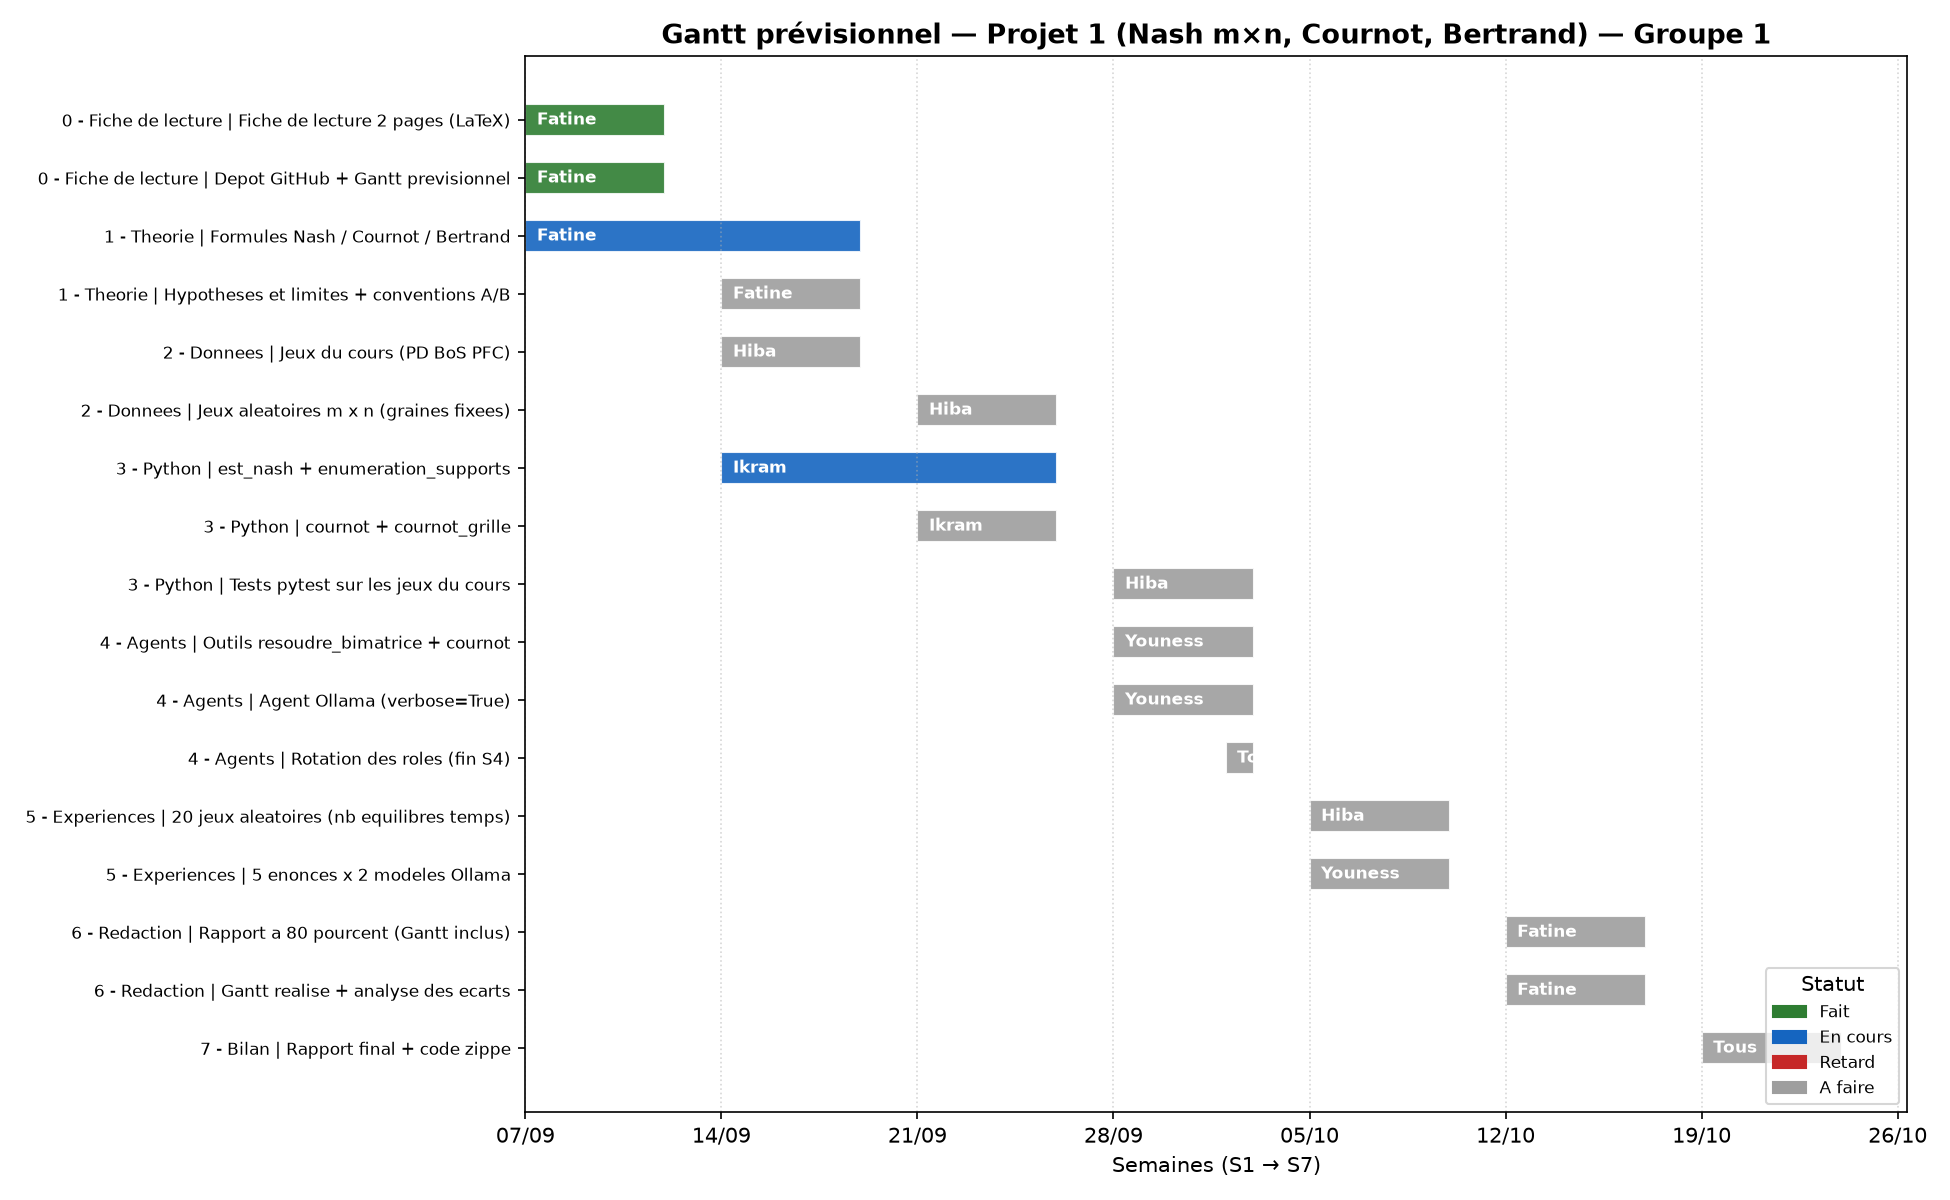
\includegraphics[width=\linewidth]{gantt_previsionnel.png}
  \caption{Gantt prévisionnel du projet (7 semaines).}
\end{figure}

\subsection{Gantt réalisé et analyse des écarts}
\begin{figure}[h]
  \centering
  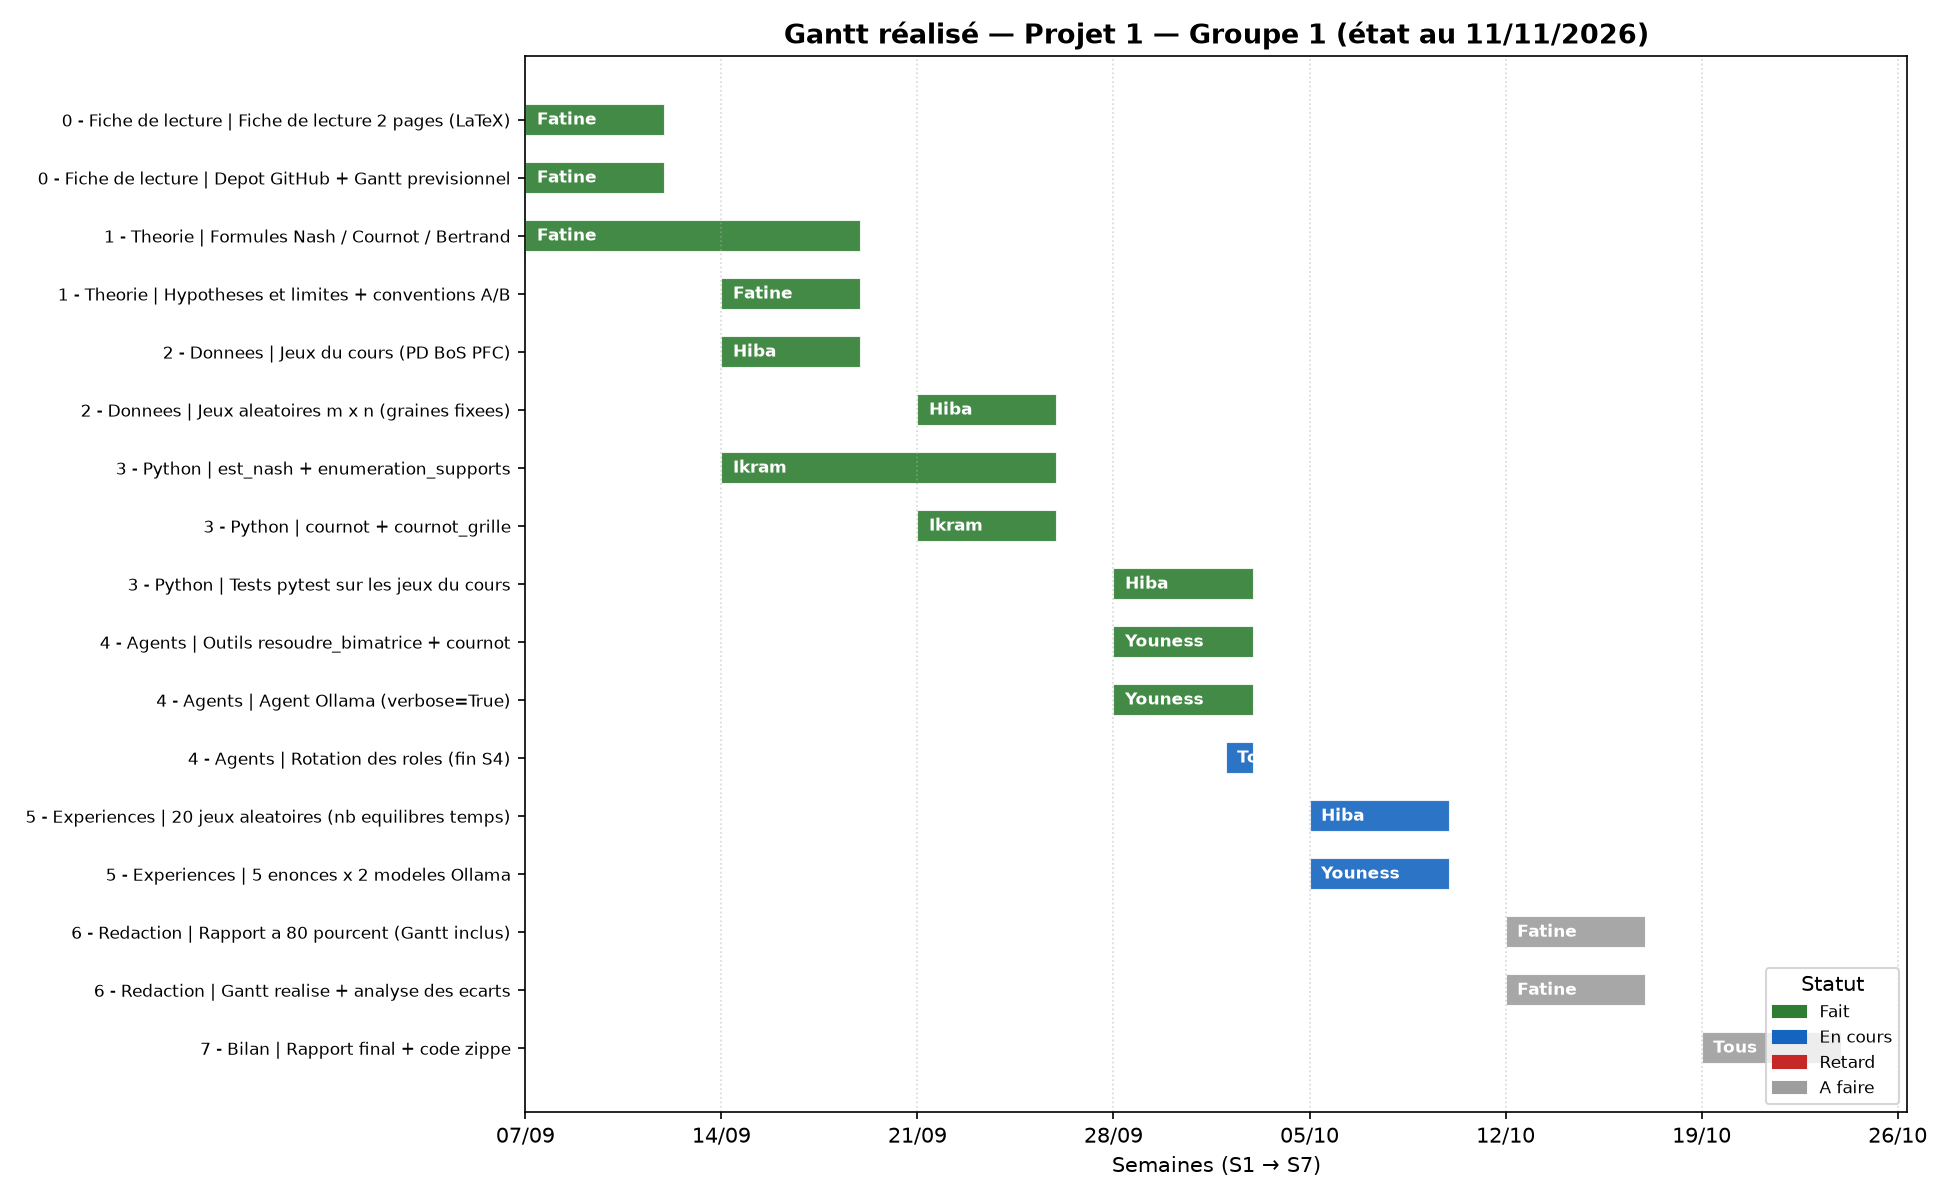
\includegraphics[width=\linewidth]{gantt_realise.png}
  \caption{Gantt réalisé (état au 11/11/2026).}
\end{figure}

\noindent\textbf{Analyse des écarts.} Les phases 0 à 4 (cadrage, théorie, données, code
Python, outils agent) sont \emph{terminées} et non plus seulement planifiées : le code des
jeux du cours est reproduit, les tests passent et l'agent LangChain réel fonctionne déjà,
alors que le plan situait l'agent en S4. Autrement dit, la partie technique a été
\emph{avancée} par rapport au prévisionnel, ce qui a dégagé du temps pour la phase
d'expériences (S5). Seules les phases 5 (expériences agents) et 6--7 (rédaction, bilan)
restent en cours ou à faire. Aucun retard bloquant n'est à signaler ; la seule difficulté
d'environnement (Python 3.15 vs \texttt{zstandard}) est documentée en annexe.

% ---------------------------------------------------------------------
\section{Théorie : formules clés, hypothèses et limites}
\subsection{Équilibre de Nash et indifférence sur les supports}
Un profil mixte $(x,y)$ est un équilibre de Nash si et seulement si
\[
(Ay)_i \le x^{\top} A y \ \ \forall i, \qquad (x^{\top}B)_j \le x^{\top} B y \ \ \forall j .
\]
Sur les supports $I=\mathrm{supp}(x)$, $J=\mathrm{supp}(y)$ avec $|I|=|J|=k$ :
\[
(Ay)_i = v_1 \ (i\in I), \qquad (x^{\top}B)_j = v_2 \ (j\in J), \qquad
\textstyle\sum_{i\in I} x_i = \sum_{j\in J} y_j = 1 .
\]

\subsection{Cournot et Bertrand}
\[
q_i=\frac{a-c-b\sum_{j\ne i} q_j}{2b}, \qquad
q^{*}=\frac{a-c}{(n+1)b}, \qquad
\pi^{*}=\frac{(a-c)^2}{b\,(n+1)^2} .
\]
Bertrand (biens homogènes, coûts égaux $c$) : $p_1=p_2=c$, profit nul.

\subsection{Hypothèses et limites}
\textbf{Hypothèses} : jeux statiques finis à deux joueurs, à information complète et
mémoire parfaite ; matrices de gains connues ; jeux \emph{non dégénérés} (aucune ligne ou
colonne dominée de façon à créer un continuum d'équilibres). Pour Cournot : demande inverse
linéaire $P(Q)=a-bQ$ avec $a>c$, coût marginal constant $c$, biens homogènes, concurrence en
quantités et jeu simultané. Pour Bertrand : biens homogènes et coûts identiques.

\textbf{Limites} : (i) l'énumération des supports est de complexité \emph{exponentielle} en
la taille du jeu, on plafonne donc à $8\times8$ ; (ii) les calculs sont numériques, des
tolérances ($10^{-9}$) sont nécessaires pour comparer les gains et déclarer un équilibre ;
(iii) le modèle ne traite ni les jeux séquentiels (forme extensive), ni les jeux à
information incomplète (Bayésiens) ; (iv) l'agent LLM peut mal traduire un énoncé, ce qui
constitue une source d'erreur distincte du solveur (voir §6.3).

% ---------------------------------------------------------------------
\section{Méthodologie}
\subsection{Fonctions pures (\texttt{src/jeux.py})}
\texttt{est\_nash}, \texttt{enumeration\_supports}, \texttt{cournot}, \texttt{cournot\_grille},
\texttt{bertrand}.

\textbf{Algorithme.} Pour chaque couple de supports $I\subseteq\{1..m\}$,
$J\subseteq\{1..n\}$ de même cardinal $k$, on résout le système linéaire d'indifférence
$Ay=v_1\mathbf{1}$ sur $I$, $x^{\top}B=v_2\mathbf{1}$ sur $J$, complété par
$\sum x_i=\sum y_j=1$. La solution est retenue si $x\ge0$, $y\ge0$ et si aucune stratégie
hors support n'est profitable (condition d'\emph{équilibre} globale). \texttt{est\_nash}
vérifie a posteriori cette dernière condition, ce qui sert de garde-fou indépendant.

\textbf{Complexité.} Le nombre de couples de supports est
$\sum_{k=1}^{\min(m,n)}\binom{m}{k}\binom{n}{k}$, soit une croissance exponentielle : c'est
la raison du plafond à $8\times8$ et de l'expérience de temps de calcul en §6.1.

\subsection{Tests (\texttt{tests/}, pytest)}
25 tests au total. Ils couvrent : (i) les \emph{jeux du cours} — dilemme du prisonnier
(1 équilibre pur), bataille des sexes (2 purs + 1 mixte), pierre-feuille-ciseaux
($(1/3,1/3,1/3)$) ; (ii) la propriété que \emph{toute} solution renvoyée par
\texttt{enumeration\_supports} passe \texttt{est\_nash} ; (iii) les cas d'erreur
(tailles incompatibles, dépassement de plafond) ; (iv) les \emph{outils sans LLM}
(\texttt{.invoke}) y compris la robustesse aux matrices passées en chaîne JSON et
l'exécution d'un \texttt{StructuredTool} LangChain. Les tests ne font aucun appel réseau.

\subsection{Outils agent (LangChain / Ollama)}
\texttt{resoudre\_bimatrice(A, B)} et \texttt{cournot(a, b, c, n\_firmes)}, plafonnés et en JSON.
Test \texttt{.invoke()} sans LLM (\texttt{tests/test\_hors\_ligne.py}), puis agent Ollama réel
(\texttt{src/agent\_langchain\_demo.py}, \texttt{create\_agent} + \texttt{ChatOllama}).

\textbf{Robustesse aux entrées du LLM.} Deux écueils ont été rencontrés et corrigés :
(i) \texttt{llama3.1} transmet parfois les matrices sous forme de \emph{chaîne}
(\texttt{"[[3, 0], [5, 1]]"}) ; le validateur pydantic de LangChain rejetait alors l'appel
\emph{avant} l'exécution, corrigé par le type \texttt{Matrice = Union[list, str]} et un
décodage \texttt{json.loads} (jamais \texttt{eval}, Règle n°5) ; (ii) selon que LangChain est
installé ou non, un \texttt{@tool} est un \texttt{StructuredTool} (non appelable
directement) ou une simple fonction, ce que gère \texttt{\_executer\_outil}. Les arguments
exacts relevés sur les 5 énoncés sont analysés en §6.2.

% ---------------------------------------------------------------------
\section{Résultats des expériences et discussion}
\subsection{Énumération des supports : nombre d'équilibres et temps de calcul}
Protocole : 20 jeux aléatoires par taille ($m=n\in\{2,3,4\}$), gains tirés uniformément
dans $[-1,1]$, graines fixées (\texttt{np.random.default\_rng}) pour la reproductibilité.
On relève le nombre d'équilibres trouvés et le temps d'exécution de
\texttt{enumeration\_supports} (tableau~\ref{tab:exp} et figure~\ref{fig:exp}).

\begin{table}[h]
\centering
\caption{Résultats sur 20 jeux aléatoires par taille.}
\label{tab:exp}
\begin{tabular}{lrrrr}
\toprule
Taille $m=n$ & Équilibres (moy.) & Équilibres (max) & Temps moyen (ms) & Temps max (ms) \\
\midrule
2 & 1{,}10 & 3 & 0{,}90 & 1{,}52 \\
3 & 1{,}60 & 3 & 4{,}87 & 8{,}89 \\
4 & 2{,}10 & 7 & 15{,}35 & 22{,}76 \\
\bottomrule
\end{tabular}
\end{table}

\begin{figure}[h]
  \centering
  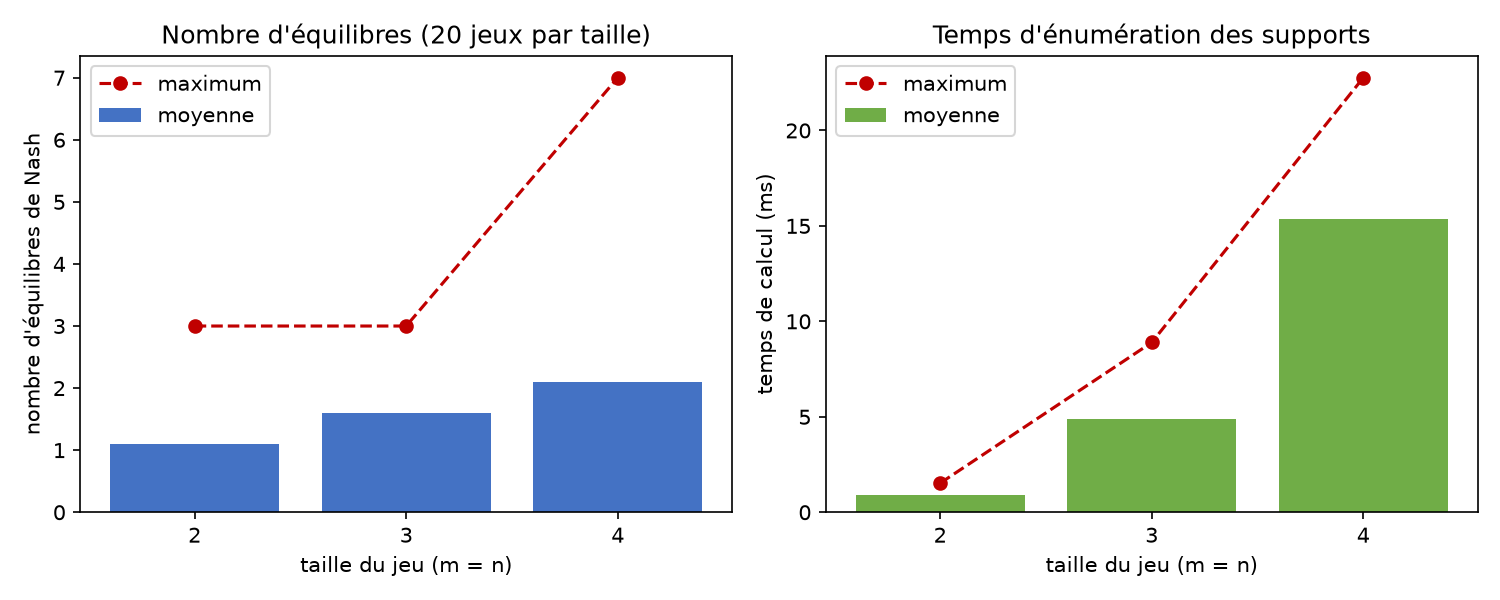
\includegraphics[width=0.95\linewidth]{fig_exp_jeux.png}
  \caption{Nombre d'équilibres et temps de calcul en fonction de la taille du jeu.}
  \label{fig:exp}
\end{figure}

\noindent\textbf{Lecture.} Le nombre d'équilibres croît avec la taille (1,1 en moyenne en
$2\times2$, 2,1 en $4\times4$) et peut atteindre 7, ce qui confirme qu'un jeu générique
admet \emph{plusieurs} équilibres et que la sélection d'équilibre est un vrai problème. Le
temps de calcul croît bien plus vite (facteur $\approx17$ entre $2\times2$ et $4\times4$),
en cohérence avec la complexité exponentielle : à $8\times8$ le solveur reste utilisable
(dixièmes de seconde) mais l'extrapolation est défavorable, d'où le plafond imposé.

\subsection{Agent : traduction des énoncés en appels d'outils}
Protocole : 5 énoncés $\times$ 2 modèles Ollama (\texttt{llama3.1} et \texttt{llama3.2:3b}),
1 répétition, température 0. Les 5 énoncés comprennent : (1) un Cournot numérique,
(2) une bimatrice $2\times2$, (3) une bimatrice $3\times3$, (4) une question
\emph{conceptuelle} (aucun outil ne doit être appelé), (5) un énoncé \emph{piège} où le coût
marginal est donné en pourcentage de l'ordonnée à l'origine. On relève l'outil appelé, la
fréquence d'appel et la présence d'une ligne « CHOIX : ».

\begin{table}[h]
\centering
\caption{Agent : appels d'outils sur 5 énoncés $\times$ 2 modèles.}
\label{tab:agent}
\begin{tabular}{lrrrrr}
\toprule
Modèle & Appels & Outil pertinent & Arguments corrects & Sans « CHOIX : » & Durée moy. (s) \\
\midrule
\texttt{llama3.1}    & 5/5 & 4/5 & 4/4 & 5/5 & 70{,}1 \\
\texttt{llama3.2:3b} & 5/5 & 4/5 & 3/4 & 5/5 & 37{,}8 \\
\bottomrule
\end{tabular}
\end{table}

\noindent{\small « Appels » = énoncés ayant déclenché un appel d'outil (sur 5) ;
« Outil pertinent » = outil attendu (4 énoncés sur 5) ; « Arguments corrects » = sur les
4 énoncés à outil ; « Sans CHOIX » = réponses n'explicitant pas la décision.}

\noindent\textbf{Observations.} Les deux modèles \emph{appellent un outil} sur les quatre
énoncés qui le justifient (Cournot, bimatrices $2\times2$ et $3\times3$, énoncé piège) et
choisissent l'outil \emph{pertinent} (\texttt{cournot} pour les énoncés économiques,
\texttt{resoudre\_bimatrice} pour les jeux matriciels). En revanche, l'examen des
\emph{arguments réels} révèle trois types d'écarts :

\begin{itemize}[nosep]
  \item \textbf{Sur-appel} : sur l'énoncé conceptuel (4), où aucune donnée n'est fournie,
        les deux modèles appellent quand même un outil. Pire, \texttt{llama3.1}
        \emph{invente} des matrices ($A=[[1,2,3],[4,5,6],[7,8,9]]$) pour satisfaire l'appel :
        c'est une hallucination de données, l'erreur la plus grave observée.
  \item \textbf{Arguments mal formés, correctement rejetés} : sur le même énoncé,
        \texttt{llama3.2:3b} envoie des listes plates ($A=[1,2,3]$) ; l'outil répond
        \texttt{\{"erreur": ...\}} au lieu de planter — le garde-fou fonctionne.
  \item \textbf{Erreur de traduction sur l'énoncé piège} : \texttt{llama3.1} convertit
        correctement $20\%$ de $100$ en $c=20$ et obtient $q^{*}=26{,}67$ ; en revanche
        \texttt{llama3.2:3b} introduit une pente fantôme ($b=0{,}2$) \emph{en plus} de
        $c=20$ et renvoie $q^{*}=133{,}33$, économiquement absurde. Le modèle 3B échoue donc
        sur l'énoncé le plus subtil.
\end{itemize}

Enfin, \textbf{aucune} des 10 réponses n'explicite sa décision par une ligne « CHOIX : »,
ce qui confirme le biais signalé dans le guide : sans relire les arguments des appels
d'outils, on ne peut pas savoir ce que le modèle a réellement décidé de faire.

\noindent\textbf{Remarque technique.} Le type \texttt{Matrice = Union[list, str]} s'est avéré
indispensable : \texttt{llama3.1} transmet les matrices $2\times2$ et $3\times3$ sous forme
de \emph{chaînes} JSON, et \texttt{cournot} reçoit parfois les scalaires en chaîne
(\texttt{"100"}, \texttt{"20"}) — convertis sans erreur par le validateur.

\subsection{Analyse des écarts à la théorie}
Trois écarts méritent d'être distingués, car ils n'ont pas la même cause :

\begin{enumerate}[nosep]
  \item \textbf{Erreur de traduction (modèle).} L'appel d'outil sur l'énoncé conceptuel — et
        surtout les matrices \emph{inventées} par \texttt{llama3.1} — sont des erreurs du LLM,
        pas du solveur : les mathématiques restent justes, c'est la décision « faut-il
        calculer, et avec quelles données ? » qui est fausse. Le guide insiste précisément sur
        ce point. Un énoncé piège mal converti ($b=0{,}2$ ajouté par le modèle 3B) produit une
        réponse numériquement cohérente mais \emph{économiquement absurde} ($q^{*}=133>a/b$) :
        la vérification par un humain reste indispensable.
  \item \textbf{Robustesse du solveur vs faiblesse du modèle.} Le solveur, lui, ne se trompe
        pas : il rejette proprement les entrées mal formées et renvoie toujours un JSON
        exploitable. Les écarts observés proviennent donc de l'interface langage naturel,
        ce qui est une conclusion importante : \emph{la qualité du résultat dépend surtout de
        la traduction de l'énoncé}, pas du calcul.
  \item \textbf{Variabilité d'exécution.} Les temps de réponse varient fortement (20 à 96 s)
        et un LLM n'est pas déterministe en pratique ; \emph{aucune conclusion ne peut être
        tirée d'une seule exécution}. C'est pourquoi le protocole fixe la graine des jeux et
        la température du modèle, et pourquoi il faudrait répéter chaque énoncé plusieurs fois
        pour estimer un taux d'erreur fiable (limite assumée de cette première campagne).
\end{enumerate}

\noindent\textbf{Bilan.} Sur cette campagne, \texttt{llama3.1} traduit correctement les
énoncés numériques mais hallucine sur l'énoncé sans données ; \texttt{llama3.2:3b} est plus
rapide mais échoue sur l'énoncé piège. Aucun des deux n'explicite sa décision. Ces résultats
plaident pour (i) un énoncé explicite dans le prompt système (« n'appelle un outil que si
des données numériques sont fournies ») et (ii) une répétition systématique des essais.

% ---------------------------------------------------------------------
\section{Conclusion et lien avec le cours}
Le projet atteint ses objectifs : le solveur $2\times2$ du cours a été généralisé en un
solveur exact $m\times n$ par énumération des supports, appliqué à Cournot et Bertrand, et
exposé à l'agent LangChain connecté au LLM local \texttt{llama3.1}. Les résultats du cours
sont reproduits exactement (dilemme, bataille des sexes, pierre-feuille-ciseaux,
$q^{*}=(a-c)/3b$), et 25 tests automatisés garantissent la non-régression.

\textbf{Apports pédagogiques.} Le projet relie trois chapitres du cours : l'équilibre de
Nash (indifférence sur les supports), les duopoles (meilleure réponse, comparaison
Cournot/cartel) et les systèmes multi-agents (outils, traduction d'un énoncé en appel de
fonction). Il met aussi en évidence une limite pratique : un LLM peut produire une
\emph{traduction fautive} d'un énoncé correct, erreur qu'aucun test du solveur ne peut
détecter.

\textbf{Prolongements} : élimination itérative des stratégies dominées pour réduire la
combinatoire, gestion des jeux dégénérés (continuum d'équilibres), extension aux jeux
séquentiels et bayésiens, et évaluation systématique de l'agent sur un jeu d'énoncés plus
large.

\appendix
\section{Reproductibilité}
Environnement : \textbf{Python 3.12 ou 3.13} (sur Python 3.15, \texttt{zstandard} n'a pas de
wheel et l'installation de LangChain échoue sans Visual C++ Build Tools) ;
\texttt{py -3.12 -m venv .venv} puis \texttt{pip install -r requirements.txt}.
Graines fixées (\texttt{np.random.default\_rng}) ; commandes : \texttt{pytest -q},
\texttt{python src/jeux.py}, \texttt{python -m src.agent\_langchain\_demo}
(ou \texttt{python -m src.agent\_demo\_ollama} sans LangChain).
Expériences : \texttt{python docs/rapport/generate\_figures.py} (jeux aléatoires) et
\texttt{python -c "from src.experiences import protocole\_agent\_ollama as p; p()"}
(agent, nécessite \texttt{ollama serve}). Données brutes : \texttt{exp\_jeux.csv},
\texttt{exp\_agent.csv}.

\end{document}
